\documentclass[aspectratio=169,11pt]{beamer}

\usepackage{iftex}
\ifXeTeX
  \usepackage{fontspec}
  \usepackage{xeCJK}
  \setmainfont{Times New Roman}
  \IfFontExistsTF{Microsoft JhengHei}{
    \setCJKmainfont{Microsoft JhengHei}
    \setCJKsansfont{Microsoft JhengHei}
    \setCJKmonofont{Microsoft JhengHei}
  }{
    \setCJKmainfont{SimSun}
    \setCJKsansfont{SimSun}
    \setCJKmonofont{SimSun}
  }
  \IfFontExistsTF{Consolas}{\setmonofont{Consolas}}{}
\fi
\usepackage{booktabs}
\usepackage{array}
\usepackage{graphicx}
\usepackage{siunitx}
\usepackage{xurl}
\usepackage{xcolor}

\usetheme{Madrid}
\usecolortheme{default}
\setbeamertemplate{navigation symbols}{}
\setbeamertemplate{footline}[frame number]
\graphicspath{{images/neural_network_fit_results/}}

\newcommand{\goodtext}[1]{\textcolor{green!45!black}{#1}}
\newcommand{\warntext}[1]{\textcolor{red!65!black}{#1}}
\newcommand{\notetext}[1]{\textcolor{blue!65!black}{#1}}
\newcommand{\pathtext}[1]{\texttt{\footnotesize\detokenize{#1}}}
\newcolumntype{L}[1]{>{\raggedright\arraybackslash}p{#1}}
\newcolumntype{R}[1]{>{\raggedleft\arraybackslash}p{#1}}

\title[NN Fitting Results]{神经网络拟合结果}
\subtitle{最佳 Stage-3 refinement、ablation 对比与轨迹级失效模式}
\author{Linan Jiang}
\institute{Aalto University}
\date{18 April 2026}

\begin{document}

\begin{frame}
  \titlepage
\end{frame}

\begin{frame}{评估对象}
\small
\begin{block}{本组结果来源}
推理脚本读取最佳 refined student model，并在 \texttt{series\_wide\_clean} 轨迹上逐点预测 penetration mean 与 predictive standard deviation。
\end{block}

\vspace{0.35em}
\begin{tabular}{L{0.29\linewidth}L{0.62\linewidth}}
\toprule
项目 & 设置 \\
\midrule
最佳 refinement run & \pathtext{distill_cdf_onset_v2_loss_tuned_conservative_20260418_114747} \\
Teacher run & \pathtext{stage2_engineered_nll_a_only_20260410_020607} \\
Evaluation split & \texttt{clean}, time window \SIrange{0}{5}{ms} \\
Raw/KD 权重 & reliable \(0.95/0.06\), uncertain \(0.50/0.25\), teacher-only \(0.00/0.75\) \\
Shape timing & anchor/onset \SI{0.025}{ms}; d2 gate start/transition \SI{0.4}{ms}/\SI{0.2}{ms} \\
\bottomrule
\end{tabular}

\vspace{0.45em}
\footnotesize
Raw result folder: \pathtext{rmse_eval_clean_20260418_115700_distill_cdf_onset_v2_loss_tuned_conservative_20260418_114747}
\end{frame}

\begin{frame}{数据规模与最佳整体误差}
\small
\begin{columns}[T,onlytextwidth]
\begin{column}{0.48\linewidth}
\begin{tabular}{L{0.55\linewidth}R{0.32\linewidth}}
\toprule
Metric & Value \\
\midrule
CSV files & 266 \\
Trajectories & 14,972 \\
Prediction points & 399,738 \\
Truth range & \SIrange{0.00}{95.88}{mm} \\
\midrule
RMSE & \SI{6.60}{mm} \\
MAE & \SI{4.81}{mm} \\
Bias & \SI{-0.40}{mm} \\
Median absolute error & \SI{3.52}{mm} \\
P90 / P95 absolute error & \SI{10.92}{mm} / \SI{13.91}{mm} \\
Range-normalized RMSE & 6.88\% \\
\bottomrule
\end{tabular}
\end{column}

\begin{column}{0.48\linewidth}
\begin{block}{相对 4/16 baseline 的变化}
\footnotesize
\begin{itemize}
  \item \goodtext{RMSE 改善}：\SI{6.90}{mm} \(\rightarrow\) \SI{6.60}{mm}。
  \item \goodtext{MAE 改善}：\SI{5.16}{mm} \(\rightarrow\) \SI{4.81}{mm}。
  \item \goodtext{低估 bias 明显减弱}：\SI{-1.29}{mm} \(\rightarrow\) \SI{-0.40}{mm}。
  \item \notetext{不确定性覆盖率也改善}：1\(\sigma\)/2\(\sigma\) = 73.56\%/96.93\%。
\end{itemize}
\end{block}

\begin{block}{不确定性}
\footnotesize
\begin{itemize}
  \item Mean predicted \(\sigma\): \SI{6.40}{mm}
  \item 1\(\sigma\) coverage: 73.56\%
  \item 2\(\sigma\) coverage: 96.93\%
\end{itemize}
\end{block}
\end{column}
\end{columns}
\end{frame}

\begin{frame}{Predicted vs. Measured Penetration}
\begin{columns}[T,onlytextwidth]
\begin{column}{0.55\linewidth}
  \centering
  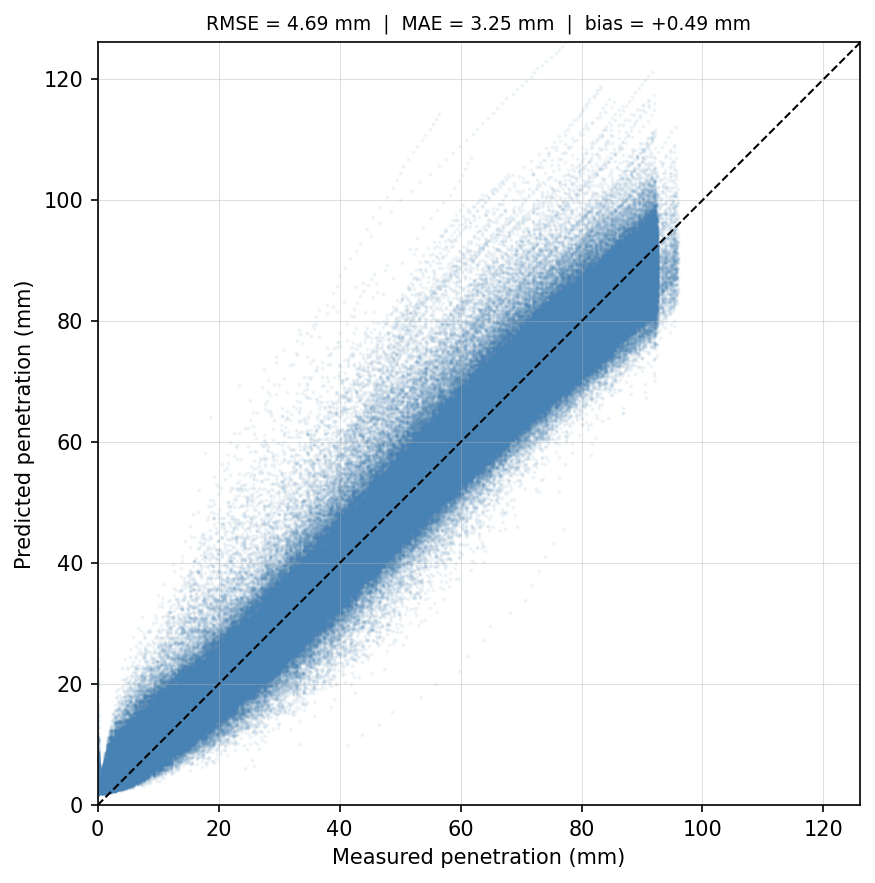
\includegraphics[width=\linewidth,height=0.73\textheight,keepaspectratio]{pred_vs_actual_best.png}
\end{column}
\begin{column}{0.41\linewidth}
\footnotesize
\begin{block}{主要观察}
\begin{itemize}
  \item loss tuning 后，主体点云仍然沿 \(y=x\) 分布。
  \item 相比 baseline，系统性低估问题明显减弱。
  \item 高 penetration 和高方差工况仍存在尾部散点，因此还需要轨迹级 review。
\end{itemize}
\end{block}
\vspace{0.2em}
\footnotesize
图中每个点是一个 time sample；横轴为 measured penetration，纵轴为 predicted penetration。
\end{column}
\end{columns}
\end{frame}

\begin{frame}{Residual Distribution 与校准}
\begin{columns}[T,onlytextwidth]
\begin{column}{0.56\linewidth}
  \centering
  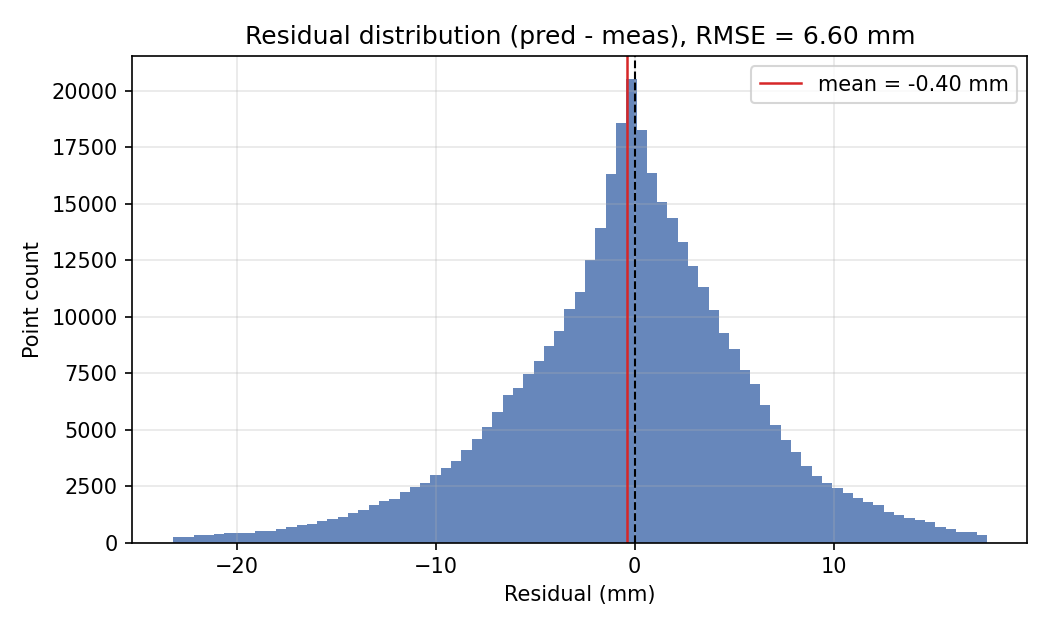
\includegraphics[width=\linewidth,height=0.72\textheight,keepaspectratio]{residual_histogram_best.png}
\end{column}
\begin{column}{0.40\linewidth}
\footnotesize
\begin{block}{Residual 定义}
\[
e = \hat{y}_{\mathrm{pen}} - y_{\mathrm{pen}}
\]
\end{block}

\begin{itemize}
  \item Bias = \SI{-0.40}{mm}，整体 under-prediction 已经明显减弱。
  \item 1\(\sigma\) coverage = 73.56\%，相对 Gaussian reference 略保守。
  \item 2\(\sigma\) coverage = 96.93\%，同样略保守，但适合筛查高风险轨迹。
  \item 校准与平均误差指标同时改善。
\end{itemize}
\end{column}
\end{columns}
\end{frame}

\begin{frame}{Ablation 对比}
\begin{columns}[T,onlytextwidth]
\begin{column}{0.63\linewidth}
  \centering
  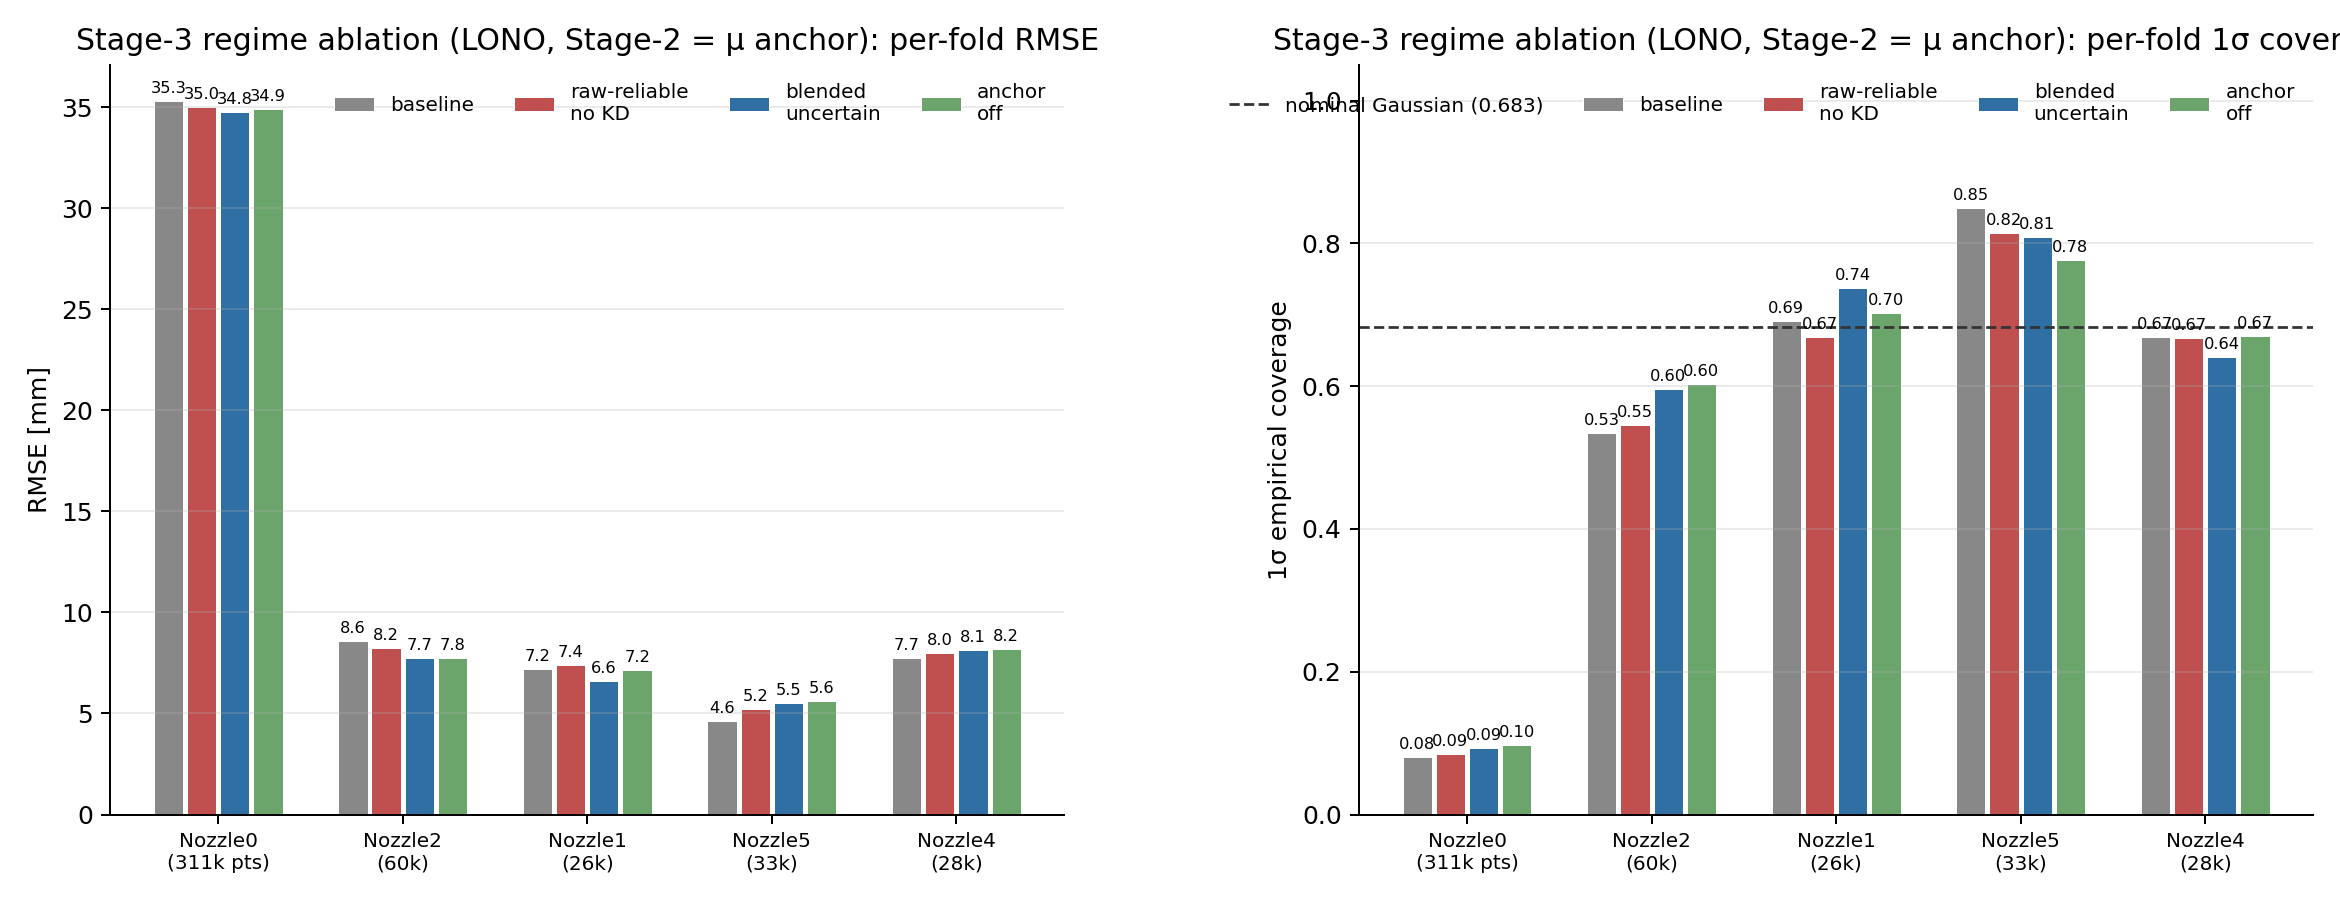
\includegraphics[width=\linewidth,height=0.68\textheight,keepaspectratio]{ablation_comparison_best.png}
\end{column}
\begin{column}{0.34\linewidth}
\scriptsize
\begin{tabular}{L{0.50\linewidth}R{0.18\linewidth}R{0.18\linewidth}}
\toprule
Run & RMSE & Bias \\
\midrule
Baseline & 6.90 & -1.29 \\
Reliable KD off & 6.88 & -1.45 \\
Anchor off & 6.76 & -0.95 \\
Uncertain raw+KD down & 6.83 & -0.70 \\
Tuned v1 & 6.64 & -0.55 \\
\goodtext{Best tuned} & \goodtext{6.60} & \goodtext{-0.40} \\
d2 back & 6.66 & -0.59 \\
\bottomrule
\end{tabular}

\vspace{0.4em}
\footnotesize
\begin{itemize}
  \item 降低 reliable raw bins 中的 KD 权重，是修正 bias 的关键方向。
  \item raw/KD reweighting 与更短的 onset anchor 组合后，得到最佳整体结果。
  \item d2 gate 回退能帮助部分 HZ nozzle，但会损失 DS300 和 overall RMSE。
\end{itemize}
\end{column}
\end{columns}
\end{frame}

\begin{frame}{最佳模型如何改变 DS300}
\begin{columns}[T,onlytextwidth]
\begin{column}{0.62\linewidth}
  \centering
  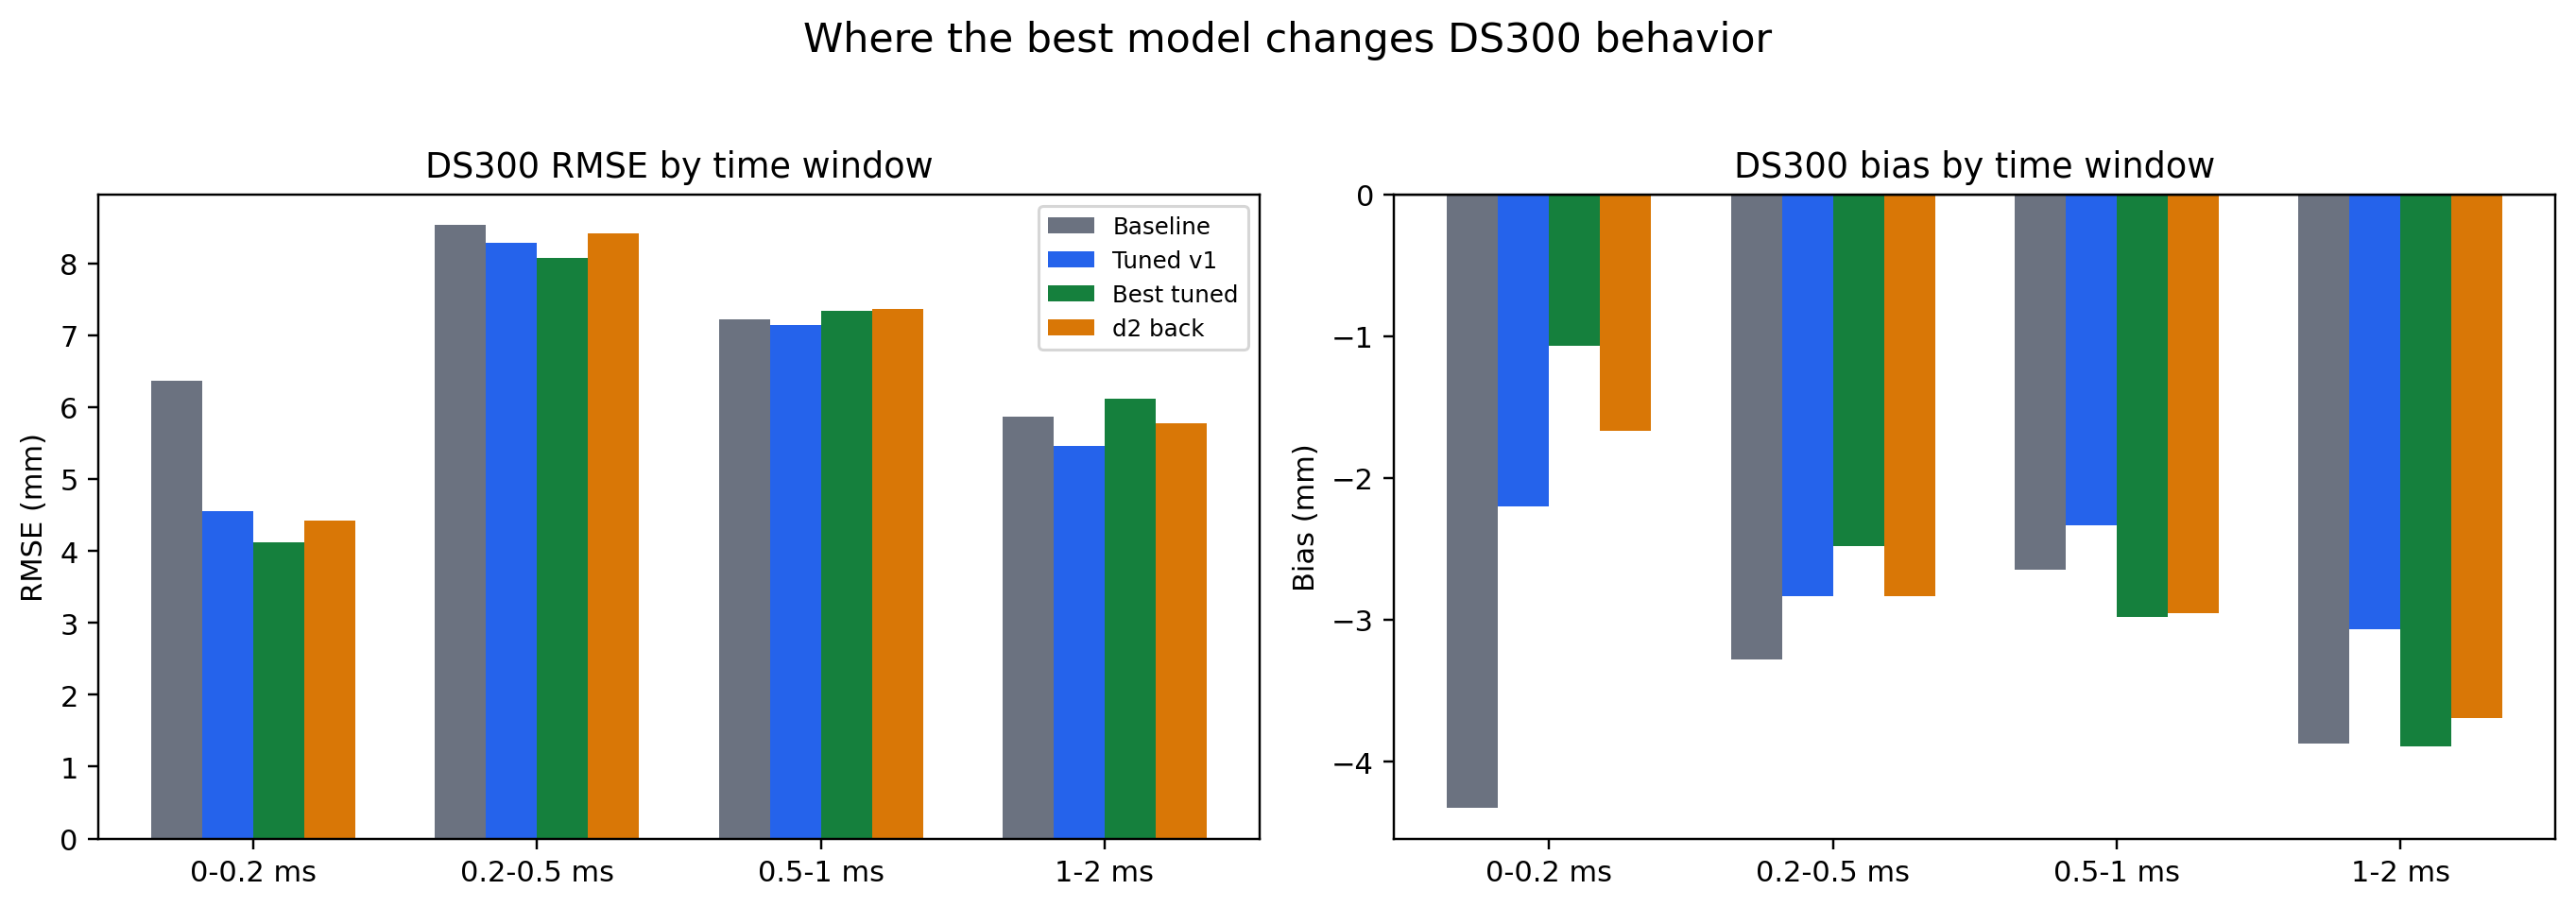
\includegraphics[width=\linewidth,height=0.68\textheight,keepaspectratio]{ds300_time_change_best.png}
\end{column}
\begin{column}{0.34\linewidth}
\footnotesize
\begin{block}{DS300 变化}
\begin{itemize}
  \item DS300 mean RMSE: \SI{6.77}{mm} \(\rightarrow\) \SI{6.12}{mm}.
  \item DS300 MAE: \SI{5.99}{mm} \(\rightarrow\) \SI{5.25}{mm}.
  \item DS300 bias: \SI{-3.36}{mm} \(\rightarrow\) \SI{-2.35}{mm}.
\end{itemize}
\end{block}

\begin{itemize}
  \item 最大收益出现在 \SIrange{0}{0.2}{ms}，即 SOI 初期低估被明显拉回。
  \item \SIrange{0.5}{2.0}{ms} 仍暴露 curvature regularization 的 trade-off。
\end{itemize}
\end{column}
\end{columns}
\end{frame}

\begin{frame}{Loss tuning 后的 per-folder trade-off}
\begin{columns}[T,onlytextwidth]
\begin{column}{0.59\linewidth}
  \centering
  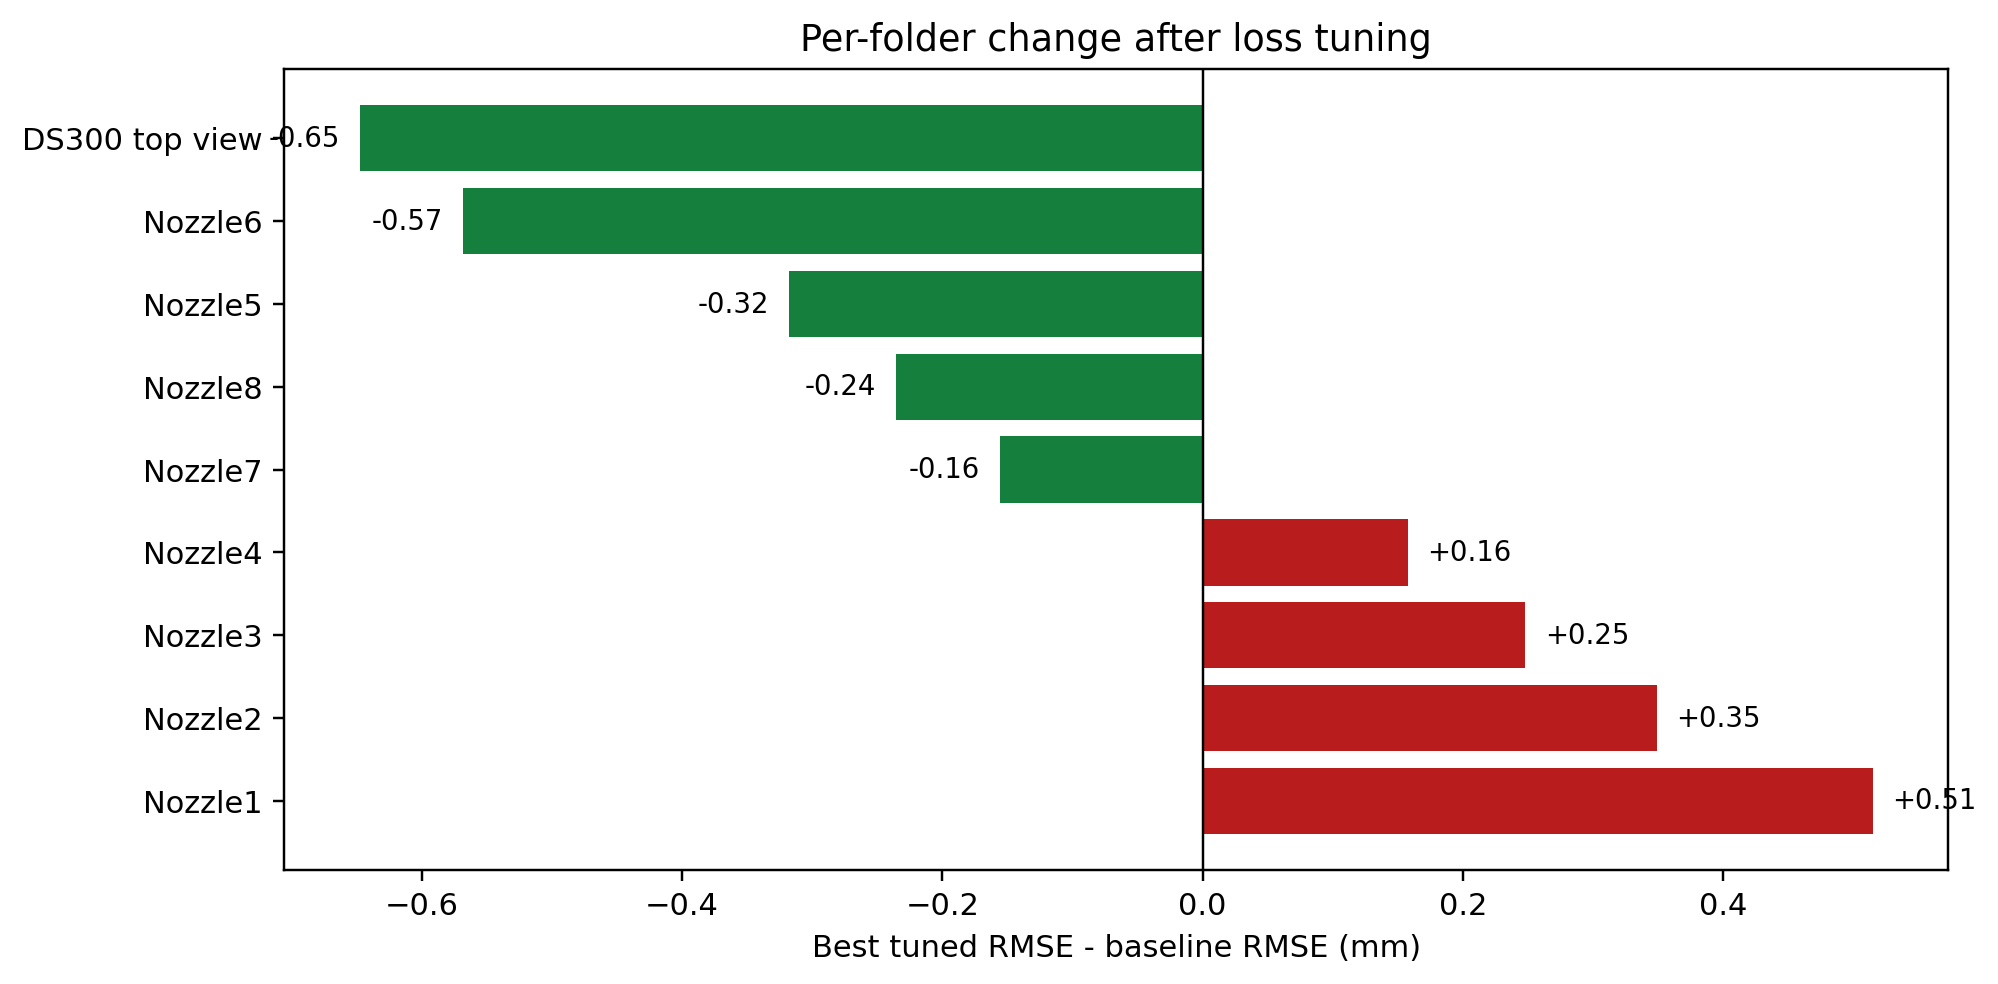
\includegraphics[width=\linewidth,height=0.68\textheight,keepaspectratio]{per_folder_delta_best_vs_baseline.png}
\end{column}
\begin{column}{0.37\linewidth}
\scriptsize
\begin{tabular}{L{0.58\linewidth}R{0.25\linewidth}}
\toprule
Folder & Best RMSE \\
\midrule
Nozzle7 & \SI{3.52}{mm} \\
Nozzle5 & \SI{3.63}{mm} \\
Nozzle6 & \SI{4.65}{mm} \\
Nozzle8 & \SI{4.81}{mm} \\
Nozzle4 & \SI{5.40}{mm} \\
Nozzle1 & \SI{5.73}{mm} \\
DS300 top view & \SI{6.12}{mm} \\
Nozzle2 & \SI{6.75}{mm} \\
Nozzle3 & \SI{9.21}{mm} \\
\bottomrule
\end{tabular}

\vspace{0.3em}
\footnotesize
\begin{itemize}
  \item 最佳 run 明显改善 DS300、Nozzle5/6/7/8。
  \item Nozzle1/2/3/4 显示跨喷嘴 trade-off，可能与几何相关的 SOI 初期加速模式有关。
\end{itemize}
\end{column}
\end{columns}
\end{frame}

\begin{frame}{最好情况：Nozzle7 / T19}
\begin{columns}[T,onlytextwidth]
\begin{column}{0.62\linewidth}
  \centering
  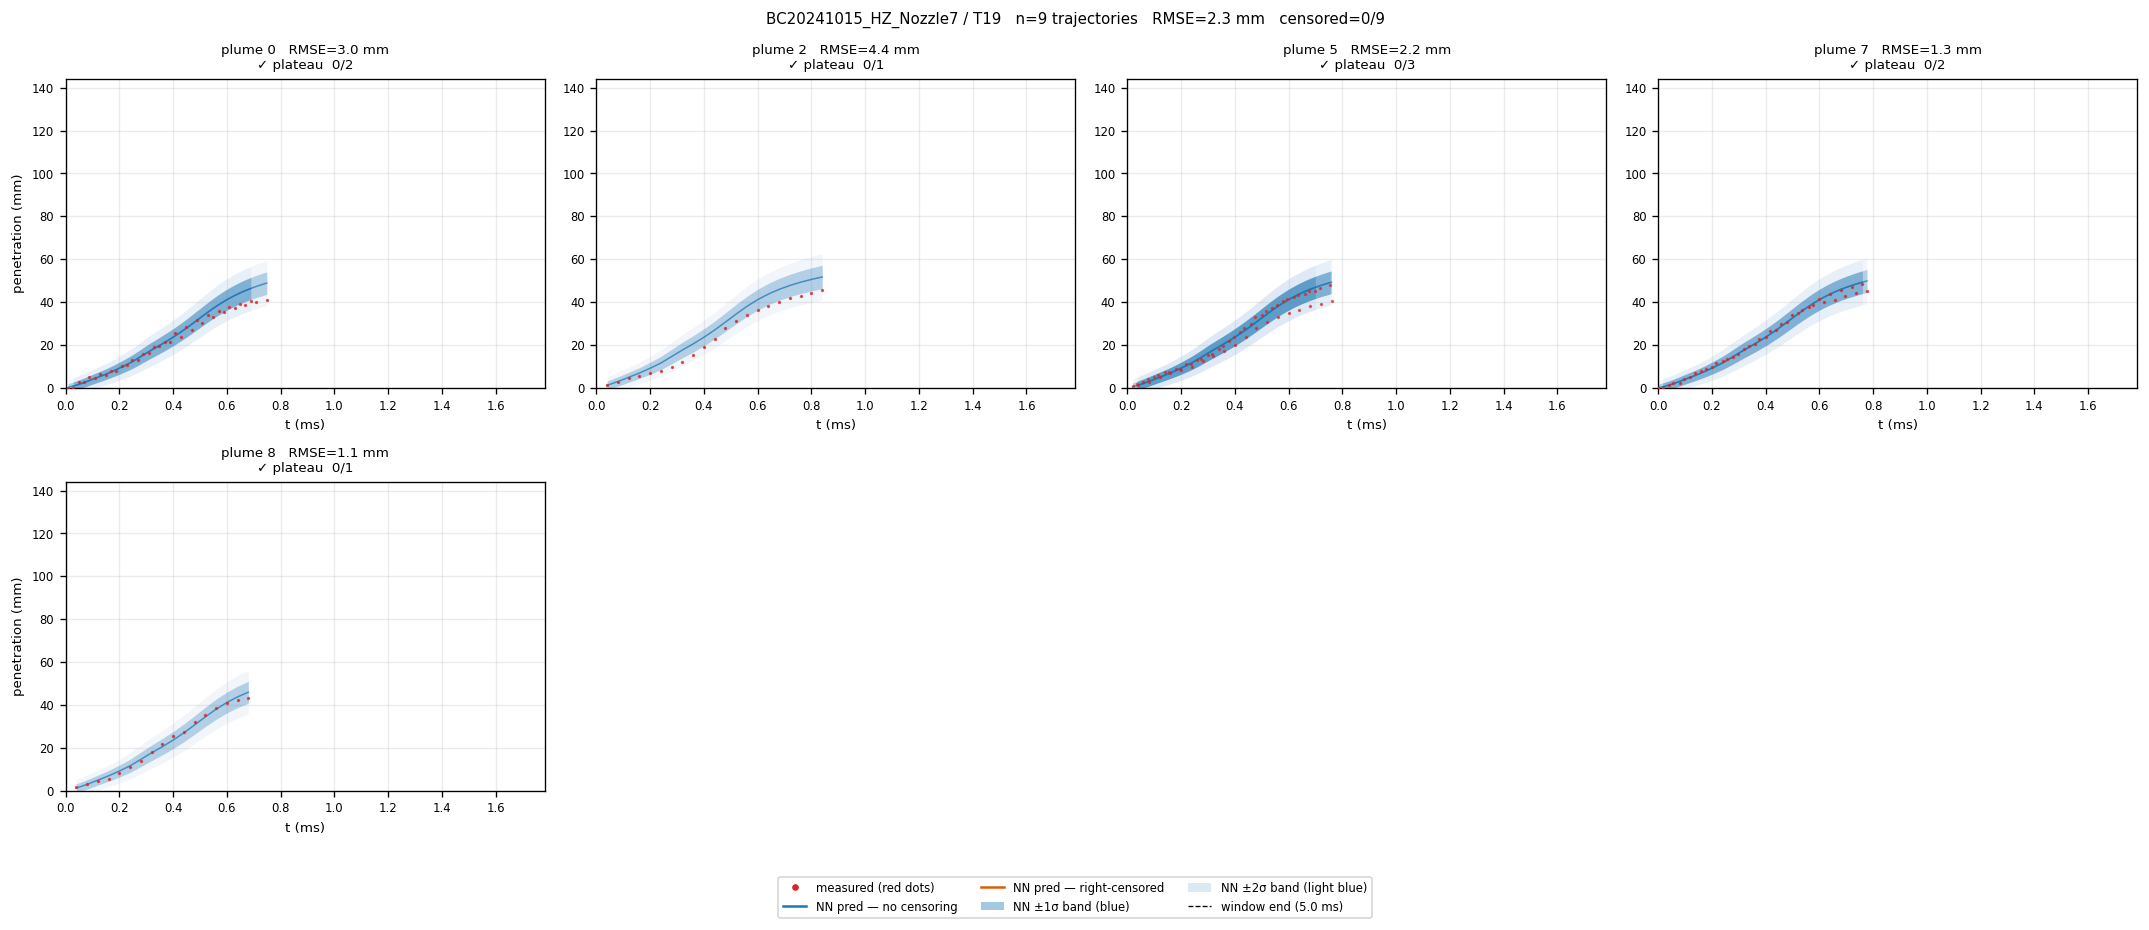
\includegraphics[width=\linewidth,height=0.62\textheight,keepaspectratio]{traj_best_nozzle7_T19.png}
\end{column}
\begin{column}{0.34\linewidth}
\footnotesize
\begin{block}{代表性特征}
\begin{itemize}
  \item Folder mean RMSE: \SI{3.52}{mm}
  \item 该组最佳 trajectory RMSE: \SI{0.47}{mm}
  \item Folder 1\(\sigma\)/2\(\sigma\) coverage: 85.63\% / 97.93\%
\end{itemize}
\end{block}

\begin{itemize}
  \item mean trend 与 plume-to-plume spread 都被较好捕捉。
  \item uncertainty band 略保守，但很实用。
  \item 这是 tuned loss 稳定 refinement、没有过修正的代表案例。
\end{itemize}
\end{column}
\end{columns}
\end{frame}

\begin{frame}{最坏情况：Nozzle3 / T3}
\begin{columns}[T,onlytextwidth]
\begin{column}{0.62\linewidth}
  \centering
  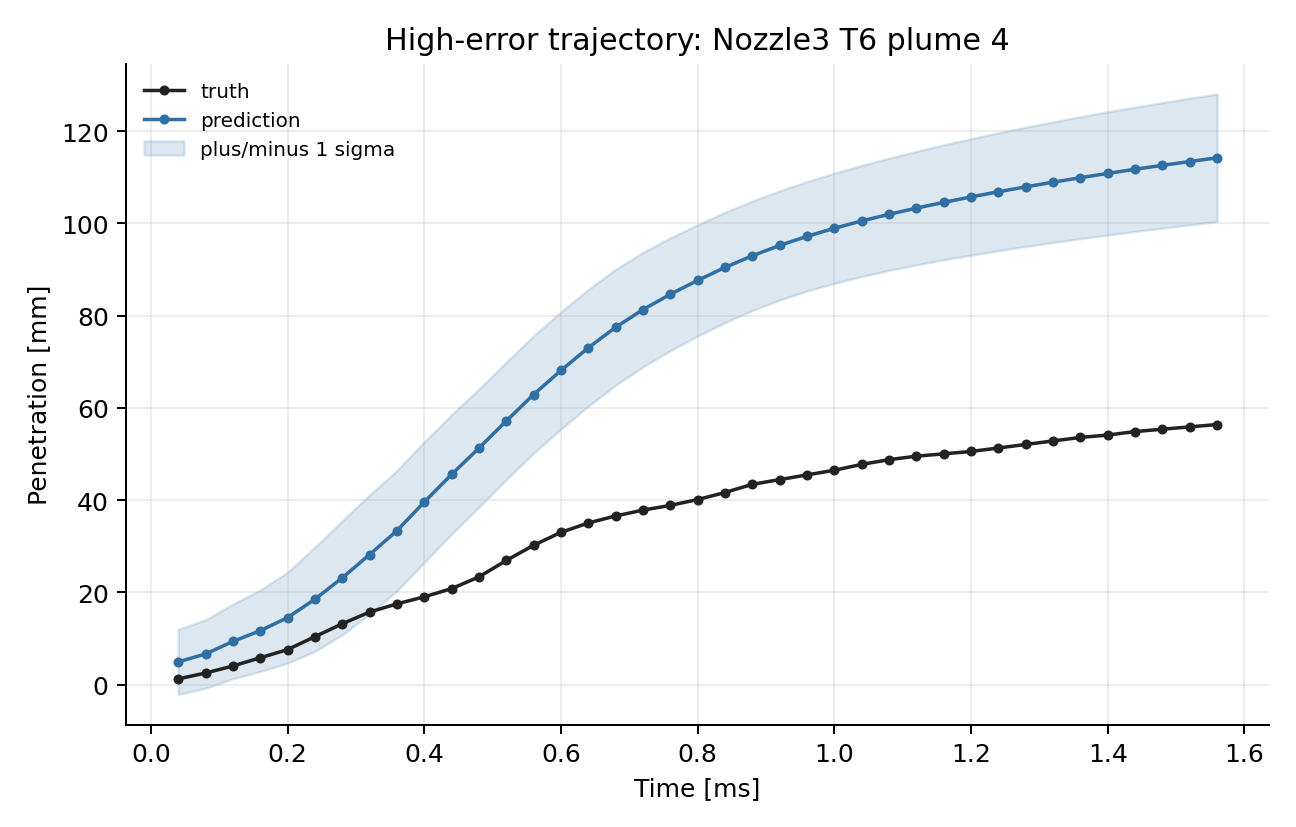
\includegraphics[width=\linewidth,height=0.62\textheight,keepaspectratio]{traj_worst_nozzle3_T3.png}
\end{column}
\begin{column}{0.34\linewidth}
\footnotesize
\begin{block}{风险信号}
\begin{itemize}
  \item Folder mean RMSE: \SI{9.21}{mm}
  \item Worst trajectory RMSE: \SI{24.33}{mm}
  \item Worst-trajectory 1\(\sigma\) coverage: 8.3\%
\end{itemize}
\end{block}

\begin{itemize}
  \item global loss tuning 不能消除所有 nozzle-family-specific failure modes。
  \item Nozzle3 在 tuning 后仍是最困难的 folder。
  \item 这支持后续研究 geometry-aware prior 或 nozzle-conditioned loss scheduling。
\end{itemize}
\end{column}
\end{columns}
\end{frame}

\begin{frame}{结论}
\small
\begin{enumerate}
  \item \goodtext{Tuned Stage-3 run 是目前最佳结果}：RMSE 为 \SI{6.60}{mm}，MAE 为 \SI{4.81}{mm}，NRMSE 为 6.88\%。
  \item \goodtext{主要系统性问题被削弱}：global bias 从 \SI{-1.29}{mm} 改善到 \SI{-0.40}{mm}；DS300 bias 从 \SI{-3.36}{mm} 改善到 \SI{-2.35}{mm}。
  \item \notetext{Ablation 支持 KD-dominance 假设}：deterministic raw-supported bins 中过强 KD 会把 teacher bias 传给 student；降低 KD 并恢复 raw supervision 能改善 DS300。
  \item \warntext{剩余误差具有喷嘴几何依赖性}：Nozzle3 和部分 HZ nozzles 与 DS300 之间存在 trade-off，说明 early-SOI acceleration 和 curvature prior 可能需要 nozzle-aware 设计。
\end{enumerate}

\vspace{0.5em}
\begin{block}{可写入论文的短结论}
本轮 loss tuning 不只是数值超参数搜索；它揭示了 raw deterministic observations 与 teacher distillation 之间的 supervision conflict，也暴露了不同喷嘴族群在 SOI 初期喷雾加速行为上的差异。
\end{block}
\end{frame}

\begin{frame}{文件索引}
\small
\begin{tabular}{L{0.28\linewidth}L{0.60\linewidth}}
\toprule
内容 & 文件 \\
\midrule
Slides source & \pathtext{Thesis/neural_network_fit_results_slides_zh.tex} \\
Compiled PDF & \pathtext{Thesis/neural_network_fit_results_slides_zh.pdf} \\
Copied/generated figures & \pathtext{Thesis/images/neural_network_fit_results/} \\
Best result folder & \pathtext{rmse_eval_clean_20260418_115700_distill_cdf_onset_v2_loss_tuned_conservative_20260418_114747} \\
Ablation CSV & \pathtext{ablation_summary_for_slides.csv} \\
DS300 time-bin CSV & \pathtext{ds300_time_bins_for_slides.csv} \\
\bottomrule
\end{tabular}
\end{frame}

\end{document}
